\section{Introduction}

Aerosols play an important role in regulating climate change. In the context of global climate change, this regulation is global. To understand the impact of aerosols on global climate change, global aerosol observations are urgently needed.

At present, the observation data of aerosols are still scattered in a large number of documents and other types of storage media. For readers who need data, it is a cumbersome and unpleasant process to move between data platforms. Moreover, the traditional literature review is fixed in the form of papers. For the author, it is necessary to read a large amount of literature for statistical compilation, and every few years need to be updated to ensure the real-time statistical knowledge of such documents. The workload is large and cumbersome. For the reader, in order to quickly acquire such statistical knowledge, it is necessary to search for the review literature and judge their authority. The acquired knowledge is also limited by the region, year, etc. that the author wants to display.

In the face of a large number of intricate data, relying on traditional literature collection methods, it is difficult to extract aerosol data in massive documents quickly and efficiently, and the practice of reviewing for many years is far from satisfying the data iteration. In this article, we will present a solution to the problem by building an aerosol knowledge base. And on the basis of the establishment of the knowledge base, we have built the world's first comprehensive literature knowledge online website system dedicated to the aerosol field, giving full play to the role of literature data.

This article is divided into six parts to introduce this website system, the first section: related work; the second section: knowledge base design; the third section: knowledge service design; the fourth section: user experience: the fifth section: data expansion; Section: Conclusion.

\section{Related Wprk}
Our work intends to leverage the knowledge and services of the literature data, and we have built the world's first comprehensive online knowledge website system for the aerosol field. These technologies have attracted many efforts from different research fields. In this section, we will review the work in each area, as our work is inspired by the literature and draws lessons from previous methods.


\subsection{Knowledge Base}

Since 2002, R.Crow first proposed the concept of Institutional Repository (IR) to actively build institutional knowledge bases in universities and institutions libraries at home and abroad. It has been nearly 16 years, but the development of knowledge base is still trying. And groping, there is no ready-made road map. This is also a big problem that the system needs to solve in the design.

At present, the commonly used knowledge bases in China include Zhiwang, Wanfang, Baidu Academic, and the knowledge bases of major universities. There are Web of science and Nature in the world. However, most of them only provide the functions of paper search and keyword indexing. Some domestic websites can provide services for checking papers. However, such data search methods are too broad, and they cannot quickly acquire a certain field in a certain period of time. Data trends within and statistical analysis results. This is exactly what we are trying to solve.

\subsection{Knowledge Service Model}
The current society is a service-based society, and the product production economy is gradually transformed into a service economy. The traditional innovation model based on technology is shifting from a user vision. We should also shift our product-centricity to users’ center.

\subsection{Crowdsourcing}
The crowdsourcing method can recruit mass participants through the Internet to complete the work that the machine is difficult to accomplish. Since Howe proposed the concept of crowdsourcing in 2006, the research and application of crowdsourcing has developed rapidly. Due to the diverse backgrounds, low labor costs, and fast task completion, crowdsourcing has developed rapidly and is widely used in image classification, manufacturing, film and television, human-computer interaction, and medicine.

In this article, we will also apply the crowdsourcing method, invite experts and scholars to fill out and submit the data of published articles, so as to expand the database.

\section{IR DESIGN}
The construction of IR requires good management, requires continuous planning, prioritization and coordination of different stakeholders, including academic and academic researchers, libraries, institutional managers, publishers, and even students participating in research (doctors, masters) benefits.

The existence of IR must meet the needs of all parties involved. For this system, we plan, prioritize and coordinate different stakeholders, including experts in academic fields, teaching and research personnel in institutions, students participating in research (doctors, masters), and the interests of the masses, and analyze the interests. The difference between the reality and the needs of the party. See Table 1 for details.

The current literature data of this aerosol knowledge base covers 75 core aerosol-related journals, with more than 13,000 aerosol-related literature data and more than 100,000 abstract data. The paper data covers China, South Korea, Japan, India, Africa, the United States and other countries and continents, as shown in Figure 1.

In China, the data covers Beijing, Chongqing, Xinjiang, Jiangsu Province, Anhui Province, Taiwan Province, Guangdong Province, Hubei Province, Guizhou Province, Gansu Province, and Shaanxi Province, as shown in Figure 2.

\begin{figure*}
	\centering
	\subfigure[World Map]{
		\label{fig:violin:PA}
		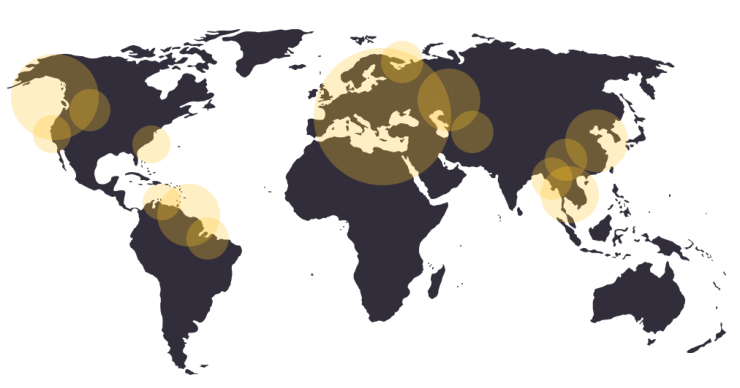
\includegraphics[width=0.4\textwidth]{figures/pic1a.pdf}
	}
	\subfigure[China Map]{
		\label{fig:violin:PB}
		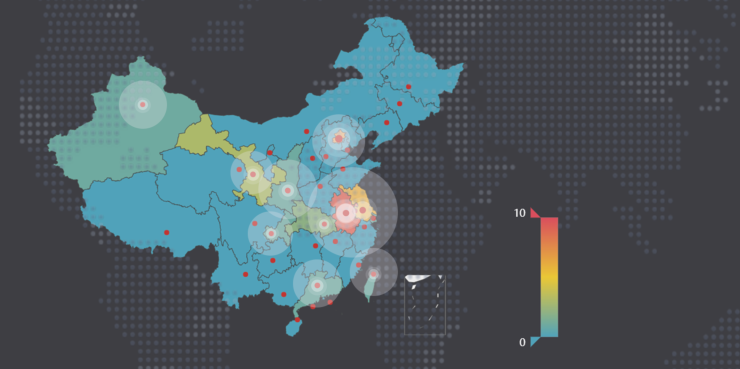
\includegraphics[width=0.4\textwidth]{figures/pic1b.pdf}
	}
\caption{Subscale.}
\end{figure*}


\section{KNOWLEDGE SERVICE}
We regard knowledge service as a system problem. Starting from the user's needs mining, through the form of questionnaires and interviews, we collect and determine the requirements, systematically apply the theory and method of design to create and plan services: system for regions, wavelengths , the year and other conditions for statistical analysis of the data in the database, and visual display, hope that users can quickly and intuitively obtain statistical knowledge of aerosol data. Services form a process and have value to end users, resulting in high quality services that enhance the user experience.

Different services have different meanings at different times, so service products are often personalized. In this regard, this paper designs adaptive service functions for the knowledge service system based on the exclusive characteristics of the aerosol literature. Therefore, after we get Table 3, we made relevant user surveys for the personnel objects in Table 3 and their interests, in order to determine the service function points.

\subsection{User Questionnaire}
We set up an online questionnaire to collect public information. A total of 20 questionnaires (currently) were collected, including 3 in the aerosol professional field and 17 in the non-aerosol professional field (both students). The questionnaire was in the form of a question. ,including but not limited to:

(1) What is the method for determining the direction of the paper before the paper is written?

(2) In what form do you want to get data in the paper?

(3) In what form do you want to judge your paper after the paper is written?

For this survey, we got a lot of important responses and suggestions. In the process of sorting out the answers, we made clear the determination of the system function. The tentative function points are as follows in Table 2:

\begin{table}
	\caption{Tentative Function Points Questionnaire}
	\label{tab:freq}
	\begin{tabular}{ll}
		\toprule
		Functions&Proportion\\
		\midrule
		Keyword Query & xx\%\\
		Topic Classification & xx\%\\
		Paper Review & xx\%\\
		Paper Evaluation & xx\%\\
		Paper Template & xx\%\\
		\bottomrule
	\end{tabular}
\end{table}

\subsection{User Interview}
In order to further deepen the user's needs and determine the system functions, we adopted the focus group interview method. We interviewed 100 volunteers, including 50 in the aerosol field (professionals include teachers and students) and 50 non-aerosol professionals (occupations include teachers, students, and other corporate workers). 

Face-to-face user interviews were conducted with a group of 10 people (the same professional). We will first set up different aerosol literature knowledge related project questions based on volunteer career information, record the problem solving needs through the discussion between volunteers, and let the volunteers click on the importance of the functions we selected before. The scale is shown in Figure 3:

\begin{figure}
	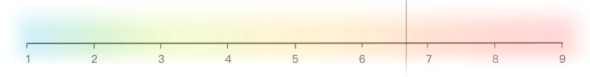
\includegraphics[width=0.45\textwidth]{figures/pic2.pdf}
	\caption{Servqual.}
\end{figure}


Based on the interview results and the scoring statistics, we removed the “paper template” function points obtained through the questionnaire, and added the “data visualization” function points obtained through focus group interviews. The final score and the determined function points are shown in Table 3:

\begin{table}
	\caption{Final Function Point and Scoring Result}
	\label{tab:freq}
	\begin{tabular}{ll}
		\toprule
		Functions&Score Result\\
		\midrule
		Keyword Query & xx\\
		Topic Classification & xx\\
		Paper Review & xx\\
		Paper Evaluation & xx\\
		\midrule
		New\\
		Data Visualization & xx\\
		\bottomrule
	\end{tabular}
\end{table}

\subsection{System Function}
Open the web page and enter the main page, as shown in Figure 3.
The system home page has 5 function entries, including:Information Search;Subject Classification;Data Crowdsourcing;Paper Check;Paper Evaluation.

Click the icon to go to the feature page. The system background image is updated randomly each time the user refreshes the main page.
The specific function operation is as follows.
\begin{figure}
	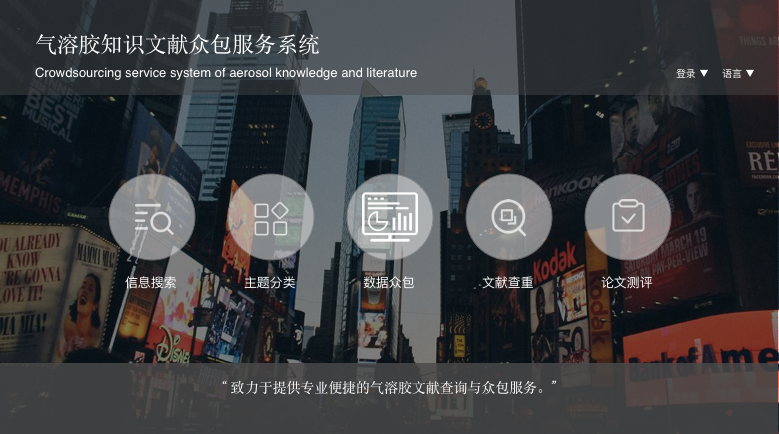
\includegraphics[width=0.35\textwidth]{figures/pic3.png}
	\caption{Main page.}
\end{figure}

\subsubsection{Information Search}
Enter the query keyword, the system will search all the documents in the database, and output all the document information containing the keywords in descending order, click to view the documents, and automatically locate the fields of the searched keywords. As shown in Figure 4.
\begin{figure}
	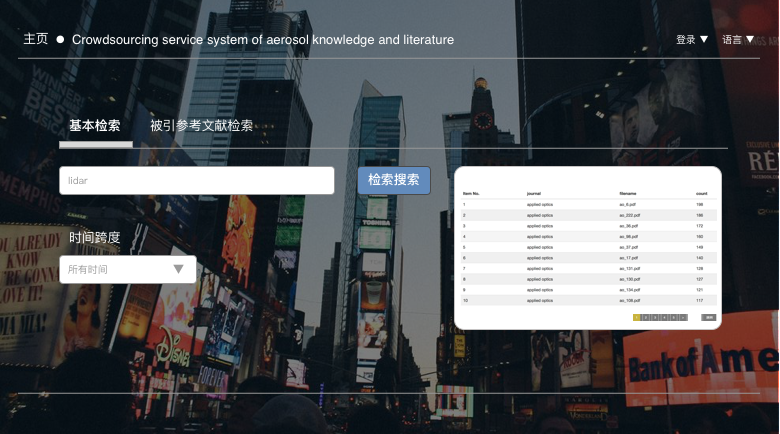
\includegraphics[width=0.35\textwidth]{figures/pic4.png}
	\caption{Information search.}
\end{figure}

\subsubsection{Subject Classification}
Users can upload documents, the system will accurately locate the document level and category, and inform the document subject classification. According to the similarity of the topic, the relevant literature is recommended for the user. The user can click to view the recommended documents. As shown in Figure 5.
\begin{figure}
	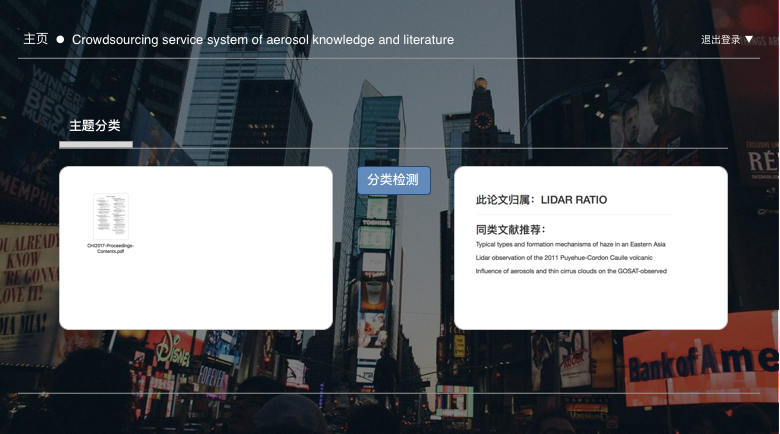
\includegraphics[width=0.35\textwidth]{figures/pic5.png}
	\caption{Subject classification.}
\end{figure}

\subsubsection{Paper Check}
Users can upload his own document and the system will upload the PDF document as the target file, perform data preprocessing such as word segmentation and deactivation, and convert it into a txt file, compare the similarity with other documents in the library, and feedback the user and upload the document. Similar published literature, users can click to view the literature, the system will automatically locate similar fields in the literature, which is convenient for users to view. As shown in Figure 6.
\begin{figure}
	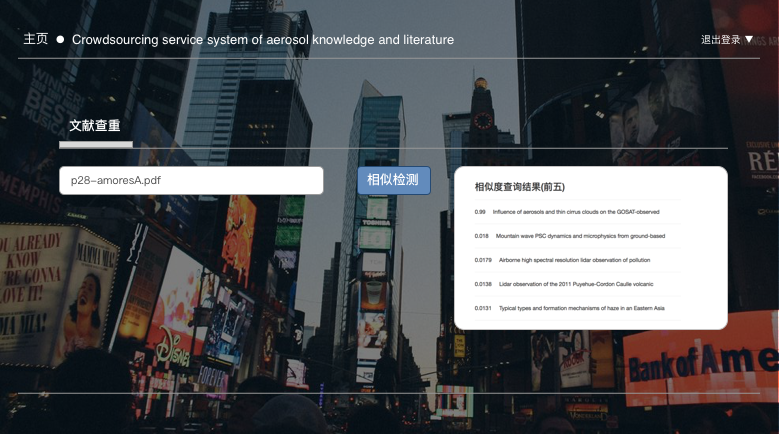
\includegraphics[width=0.35\textwidth]{figures/pic6.png}
	\caption{Paper check.}
\end{figure}

\subsubsection{Data Crowdsourcing}
See the next section for details.

\subsubsection{Paper Evaluation}
When users upload a manuscript written by themselves, the system will use the uploaded PDF document or the submitted paper information as the target files,  and compare them with the published papers or the more influential papers in the library. Finally, feedback the level of the user's target paper and recommend the corresponding excellent papers.As shown in Figure 7.
\begin{figure}
	\centering
	\subfigure[Data submission]{
		\label{fig:violin:PA}
		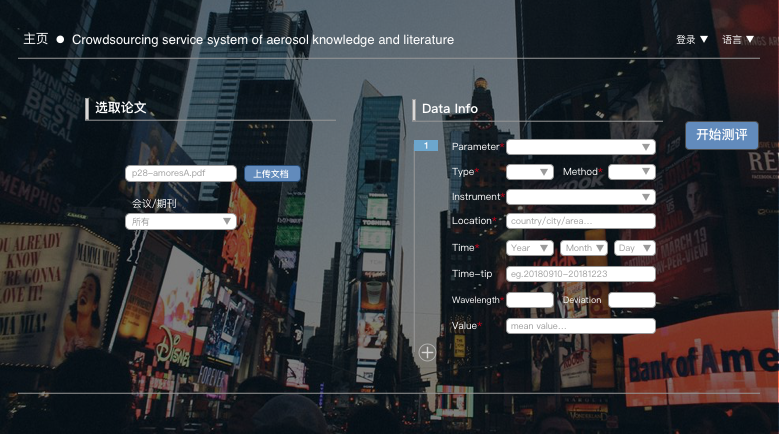
\includegraphics[width=0.35\textwidth]{figures/pic8a.png}
	}
	\subfigure[Evaluation result]{
		\label{fig:violin:PB}
		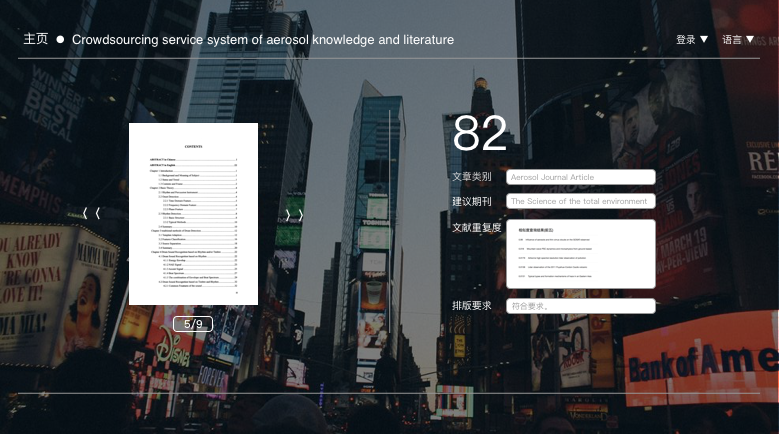
\includegraphics[width=0.35\textwidth]{figures/pic8b.png}
	}
	\caption{(a) In the [Data info] list, the user needs to fill the list with  aerosol parameter type, Method, Instrument, Location, Time, Time-tip (such as a certain time period, a certain season, etc.), Wavelength, Deviation, Value (parameter other Values, such as Mean\_value, etc.). In addition to the Time-tip and Deviation options, the rest are required information items.
	(b) On the right side of the interface, the system will give a rating item, including:Overall score; paper category; recommended journal: give the name of the journal that best meets the submission; document repeatability: list the top five documents with the highest similarity to the uploaded paper in the whole library, sorted in descending order of similarity; : Compare the paper format with the existing paper format template in the database to determine whether it meets the requirements.}
\end{figure}


\section{CROWDSOURCING AND DATA EXPANSION}
As system users continue to grow and data continues to emerge, data update iterations are a major issue that needs to be addressed. In the subsequent data collection and update of the knowledge service system in this document, we adopted a crowdsourcing method and proposed a new formatted data submission method to combine crowdsourcing submission data with data formatting storage and data analysis to achieve perfect knowledge. The role of the library and feedback user data information to ensure the update and expansion of the database.

\subsection{Parameter Setting}
After discussing with the graduate students of the Optoelectronics College Collaborative Laboratory, we designed a questionnaire experiment. The subjects were 30 graduate students in the School of Optoelectronics. The questionnaire was divided into five parts: literature publication information, aerosol basic information, optical parameter information, spatio-temporal information, and particle microphysical characteristics. The subjects were required to give these five parts separately. I think that an aerosol data related literature may contain important attributes. We compiled and merged the attributes of the 30 questionnaires collected. The results of the questionnaire included preliminary 28 attributes that would cover the important information needed. To increase the scalability, we added a “Remarks” attribute to each category. For the recording of other possible additional information, the total attribute is 33 as a paradigm preliminary attribute option, as shown in Figure 9.

In the follow-up, we further interviewed experts and scholars in the field of aerosols, taking into account the importance of the data and the clarity of the records. Finally, the attributes included in the paradigm were determined to be 17 and the four categories except the published information were combined. Into the data, the attributes contained in the paradigm are divided into article attributes and data attributes in the large class. As shown in Tables 4 and 5.

\begin{table}
	\caption{Article Attribute.}
	\label{tab:freq}
	\begin{tabular}{ll}
		\toprule
		Article Attribute&Content\\
		\midrule
		Journal & 75 journal options\\
		DOI & Unique Number of article\\
		Paper Name & Full name of the document\\
		Author & Corresponding author\\
		Unit & Company or school\\
		Tool & Observation, simulation\\
		\bottomrule
	\end{tabular}
\end{table}

\begin{table*}
	\caption{Data Attribute.}
	\label{tab:freq}
	\begin{tabular}{lp{0.7\textwidth}}
		\toprule
		Data Attribute&Content\\
		\midrule
		Key Physics Parameters & Lidar ratio, depolarization ratio, backscatter coefficient, extinction coefficient, optical depth, depolarization spectral ratio, color ratio, angstrom exponents\\
		Aerosol Type & Dust, smoke, clean continental, polluted continental, polluted dust, clean marine\\
		Method & Observation, retrival\\
		Laser Wavelength & 355, 440, 532, 645, 780, 870, 1020, 1540\\
		Address & Country, province, city\\
		Address Note & Such as a foreign country, the country specific to the school, latitude and longitude and other information\\
		Time & Year, month, day\\
		Time Note & Time interval\\
		Mean & Optical parameter average, decimal form\\
		Standard deviation & Optical parameter standard deviation, decimal form\\
		Value note & Data Interval\\
		\bottomrule
	\end{tabular}
\end{table*}

\subsection{Web Design}
The system uses the eight keywords of lidar ratio, depolarization ratio, backscatter cofficient, extinction cofficient, optical depth, depolarization spectral ratio, color ratio, angstrom exponents to guide the document information from Journal, DOI, Type, Method and so on. Extract and fill in the submission database. The specific web page information is shown in Figure 8.

In terms of user experience, in order to save user data filling time, we set the thesaurus function, set the drop-down options in multiple options such as Journal, Instrument, Type, and province cities, users can click to complete. In terms of data security, the system will automatically save the user to fill in the data to avoid data loss caused by webpage error shutdown, network disconnection and other reasons. The specifics of the user interaction experience will be covered in Section 6.

\begin{figure}
	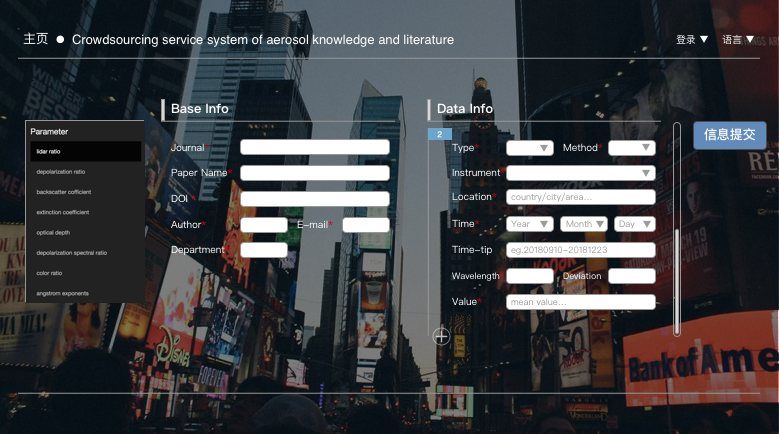
\includegraphics[width=0.35\textwidth]{figures/pic7.png}
	\caption{Website navigation.}
\end{figure}

\subsection{Crowdsourcing task organization method}
We submit data through invitations and autonomy.

By sending an email to invite experts and scholars in the aerosol field, journals and journals to submit the data of the published papers on the crowdsourcing submission page of the system, this will help improve the accuracy of the system's "paper evaluation" function. According to the format paradigm of excellent papers, we can judge the grades and advantages and disadvantages of the evaluation documents submitted by users.

Student users can get convenience from the system. After publishing the paper, we encourage and very welcome users to submit data independently and help the system to expand data.

\subsection{Automatic system update}
In addition to the background staff uploading the document data, the background of the system will automatically detect the recent literature update of each data platform, the crawler automatically downloads the document information and the abstract, promptly reminds the background personnel to update the data.

\section{USER STUDY}
We conducted an experimental test of the experience of the website. We invite volunteers who have participated in the questionnaires and interviews, as well as volunteers who have not participated in the activities related to the system, and provide us with feedback.

\subsection{System usability and usability test}
We convened the subjects who had previously interviewed to complete the system's usability and usability tests. The experimenter will experience the various functions of the system by looking up the paper information. Since our system is aimed at the field of photoelectrosols, our subjects were also professionals in the field of interviews.

Similarly, we use the subscale to let users rate the system's ease of use and usability, and make recommendations for system layout. The system usage is shown in Table 6.

\begin{table}
	\caption{Article Attribute.}
	\label{tab:freq}
	\begin{tabular}{ll}
		\toprule
		Article Attribute&Content\\
		\midrule
		Journal & 75 journal options\\
		DOI & Unique Number of article\\
		Paper Name & Full name of the document\\
		Author & Corresponding author\\
		Unit & Company or school\\
		Tool & Observation, simulation\\
		\bottomrule
	\end{tabular}
\end{table}

\subsection{System time-saving test}
... ...


\section{Conclusions}
This paper proposes a new method of data collection, storage, collation, analysis and presentation of literature, and develops a paradigm analysis and crowdsourced aerosol literature knowledge service system, which provides an effective means for collecting aerosol historical observation data and provides users with A variety of aerosol literature knowledge service functions.

At present, the system functions need to be improved. The system interaction and user experience need to be considered from the user's point of view. Through more tests, the system efficiency is improved.


\begin{acks}
	The authors would like to thank Dr. Yuhua Li for providing the
	MATLAB code of the \textit{BEPS} method.
	
	The authors would also like to thank the anonymous referees for
	their valuable comments and helpful suggestions. The work is
	supported by the \grantsponsor{GS501100001809}{National Natural
		Science Foundation of
		China}{http://dx.doi.org/10.13039/501100001809} under Grant
	No.:~\grantnum{GS501100001809}{61273304}
	and~\grantnum[http://www.nnsf.cn/youngscientists]{GS501100001809}{Young
		Scientists' Support Program}.
	
\end{acks}
